\documentclass[tikz,border=12pt]{standalone}
% Shared visual language for standalone EMT block diagrams.
\usepackage{amsmath}
\usetikzlibrary{arrows.meta,backgrounds,calc,fit,positioning}

\tikzset{
    emt diagram/.style = {>={Stealth[length=2.4mm]}},
    line/.style        = {semithick, rounded corners=6pt},
    block/.style       = {draw, semithick, fill=white,
                          minimum height=1cm, minimum width=2.3cm},
    hblock/.style      = {block, minimum width=2.24cm, minimum height=1.3cm},
    vblock/.style      = {block, minimum width=1.3cm, minimum height=2.24cm},
    sum/.style         = {draw, semithick, fill=white, circle,
                          inner sep=2.6pt},
    signal/.style      = {circle, fill, inner sep=1.4pt,
                          label distance=3pt},
    sig/.style         = {font=\small},
    pm/.style          = {font=\scriptsize},
    wire jump/.style   = {line,
                          preaction={draw=white, line width=3pt,
                                     line cap=round}},
    enclosure/.style   = {draw, dashed, semithick, rounded corners=4pt},
    operator enclosure/.style = {enclosure, inner xsep=7mm, inner ysep=6mm}
}


\begin{document}
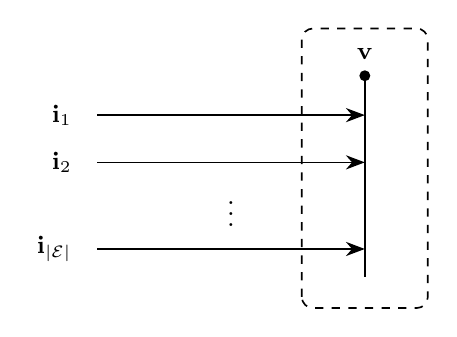
\begin{tikzpicture}[emt diagram]

% ================= Bus voltage node =================
\draw[line] (0, -1.25) -- (0, 1.3);
\node[signal, label={[sig]above:$\mathbf{v}$}] at (0, 1.3) {};

% ================= Connected-device currents =================
\coordinate (i1) at (-3.4, 0.8);
\coordinate (i2) at (-3.4, 0.2);
\coordinate (iE) at (-3.4, -0.9);

\draw[->, line] (i1) -- (0, 0.8);
\draw[->, line] (i2) -- (0, 0.2);
\draw[->, line] (iE) -- (0, -0.9);

\node[sig, anchor=east] at ($(i1)+(-0.2,0)$) {$\mathbf{i}_1$};
\node[sig, anchor=east] at ($(i2)+(-0.2,0)$) {$\mathbf{i}_2$};
\node[sig, anchor=east] at ($(iE)+(-0.2,0)$)
    {$\mathbf{i}_{|\mathcal{E}|}$};
\node at (-1.7, -0.35) {$\vdots$};

% ================= Model enclosure =================
\draw[enclosure] (-0.8, -1.65) rectangle (0.8, 1.9);

\end{tikzpicture}
\end{document}
